% DOCUMENT
\documentclass[oneside,14pt,a4paper]{extreport}

% LANGUAGE
\usepackage[T2A]{fontenc}
\usepackage[utf8]{inputenc}
\usepackage[english, ukrainian]{babel}

% \usepackage{minted}
\usepackage{pgfplots}

% VARIABLES
\newcommand \labno    {2}
\newcommand \course   {Організація наукових досліджень}
\newcommand \group    {11}
\newcommand \lecturer {Ізонін І. В.}
\newcommand \theme    {Оформлення списку літератури з використанням систем управління бібліграфічною інформацією}
\newcommand \purpose  {Встановити, налаштувати та навчитися використовувати безкоштовний бібліографічний менеджер Zotero для оформлення списку літератури у наукових роботах.}

% PACKAGES
\usepackage{amssymb}
\usepackage{amsmath}
\usepackage{multirow}
\usepackage{url}
\usepackage[unicode=true]{hyperref}
\usepackage{hanging}

% GEOMETRY
\usepackage{geometry}
\geometry{left   = 2.5cm}
\geometry{right  = 1cm}
\geometry{top    = 2cm}
\geometry{bottom = 2cm}
\renewcommand {\baselinestretch} {1.5}
\setlength\parindent{1cm}

% IMAGES
\usepackage{graphicx}
\usepackage{indentfirst}
\graphicspath{ {./imgs/} }
\usepackage{float}

% FOOTER
\usepackage{fancyhdr}
\fancyhf{}
\renewcommand{\headrulewidth}{0pt}
\cfoot{\hfill \thepage}
\pagestyle{fancy}

% CHAPTERS

\newcommand\Section[1]{
 \refstepcounter{section}
 \section*{
  \arabic{section}. #1}
}

\newcommand\Subsection[1]{
 \refstepcounter{subsection}
 \section*{
  \arabic{section}.\arabic{subsection}. #1}
}

\sloppy
\begin{document}
\begin{titlepage}

\centering
 \textbf{
  МІНІСТЕРСТВО ОСВІТИ І НАУКИ УКРАЇНИ \
  НАЦІОНАЛЬНИЙ УНІВЕРСИТЕТ \flqq{}ЛЬВІВСЬКА ПОЛІТЕХНІКА\frqq{} \
  ІНСТИТУТ КОМП’ЮТЕРНИХ НАУК ТА ІНФОРМАЦІЙНИХ ТЕХНОЛОГІЙ
 }

\vspace{0.5cm}
 \textbf{
  Кафедра систем штучного інтелекту
}

\vspace*{\fill}

  {
    \centering
    
\includegraphics[width=7cm]{imgs/logo.eps}
  }

\vspace{1cm}

  {\textbf{ЗВІТ} \par{}
  {про виконання практичної роботи №\labno}
   \par}
  {з курсу \flqq{}\course\frqq{} \par}

\vspace{1cm} \theme

\raggedleft\vfill

 {\textbf{Виконав:} \par}
 {ст. гр. КНСШ-\group \par}
 {Тимошенко Павло Олександрович \par}

% \vspace{1cm}

 {\textbf{Перевірив:} \par}
 {доцент каф. СШІ, к.т.н.,}
 {\lecturer \par}

\vspace{1cm}

\centering {Львів -- \the\year \par}

\end{titlepage}

\Section{Постановка завдання}

Далі описано пункти, які потрібно виконати у межах цієї практичної роботи.

\begin{enumerate}
    \item Ознайомитись із теоретичними відомостями, встановити браузерний та standalone-версії бібліграфічного менеджера Zotero, зареєструватись та синхронізувати їх.
    \item Написати дипломної роботи, додати кілька абзаців тексту, що стосуються тематики роботи. Відформатувати його за вимогами. В різних місцях цих абзаців, використовуючи правила цитування, поставити щонайменш шість посилань на наукові роботи, які відповідають таким вимогам:
    \begin{itemize}
        \item релевантні до тематики тексту;
        \item долучені у бібліотеку через розширення із: а) будь-якого журналу корпорації MDPI, б) видавництва Springer та в) видавництва Elsevier (3 статті);
        \item долучені у бібліотеку вручну із сервісу CEUR-WS.org (1 стаття);
        \item долучені з використанням DOI на основі бази PubMed та IEEE Xplore Digital Library (2 статті).
    \end{itemize}
    \item Сформувати бібліографію цих робіт із використанням стилів APA 7\textsuperscript{th}, Vancouver та MDPI чи якогось іншого. Описати відмінності стилів та подати список літературних джерел.
    \item Описати виконані кроки.
\end{enumerate}

\Section{Хід роботи}

В цьому розділі описано процес виконання практичної роботи та пророблені кроки. 

\Subsection{Налаштування програми}

Спершу я встановив браузерне розширення Zotero. Процес додавання продемонстровано на Рис.~\ref{pic:zotero-plugin-added} та Рис.~\ref{pic:zotero-plugin}.

\begin{figure}[H]
    \centering
    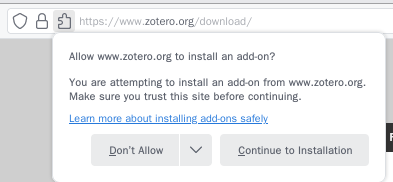
\includegraphics[width=10cm]{imgs/sp2_zotero_plugin.png}
    \caption{Надання дозволу на встановлення плагіну в браузері Mozilla Firefox.}
    \label{pic:zotero-plugin}
\end{figure}

\begin{figure}[H]
    \centering
    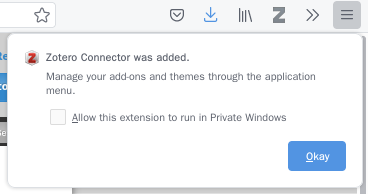
\includegraphics[width=10cm]{imgs/sp2_zotero_plugin_added.png}
    \caption{Плагін Zotero встановлено.}
    \label{pic:zotero-plugin-added}
\end{figure}

Десктопний застосунок Zotero для Linux я завантажив  у вигляді tarball-пакунку, розпакував і запустив так:

\small\begin{verbatim}
paul@paulpc:~$ mkdir ~/media/ubuntuprgs/zotero
paul@paulpc:~$ tar -xf ~/media/downloads/Zotero-5.0.96.3_linux-x86_64.tar.bz2
     -C ~/media/ubuntuprgs/zotero/
paul@paulpc:~$ ls ~/media/ubuntuprgs/zotero/
Zotero_linux-x86_64
paul@paulpc:~$ ls ~/media/ubuntuprgs/zotero/Zotero_linux-x86_64/
application.ini     libmozavutil.so   minidump-analyzer
chrome              libmozgtk.so      omni.ja
chrome.manifest     libmozsandbox.so  pdfinfo
components          libmozsqlite3.so  pdftotext
defaults            libnspr4.so       platform.ini
dependentlibs.list  libnss3.so        plugin-container
dictionaries        libnssckbi.so     plugin-container.sig
extensions          libnssdbm3.chk    poppler-data
firefox-bin.sig     libnssdbm3.so     set_launcher_icon
firefox.sig         libnssutil3.so    Throbber-small.gif
fonts               libplc4.so        updater
gmp-clearkey        libplds4.so       updater.ini
gtk2                libsmime3.so      zotero
icons               libsoftokn3.chk   zotero-bin
libfreeblpriv3.chk  libsoftokn3.so    zotero.desktop
libfreeblpriv3.so   libssl3.so        zotero.jar
liblgpllibs.so      libxul.so
libmozavcodec.so    libxul.so.sig
paul@paulpc:~$ ./media/ubuntuprgs/zotero/Zotero_linux-x86_64/zotero
\end{verbatim}\normalsize

На Рис.~\ref{pic:zotero-app-started} показано вигляд вікна програми при запуску. На Рис.~\ref{pic:zotero-connector} показано, що встановлений застосунок автоматично пов'язується із браузерним розширенням, і при створенні нової закладки у браузері вона одразу додається в застосунок.

\begin{figure}[H]
    \centering
    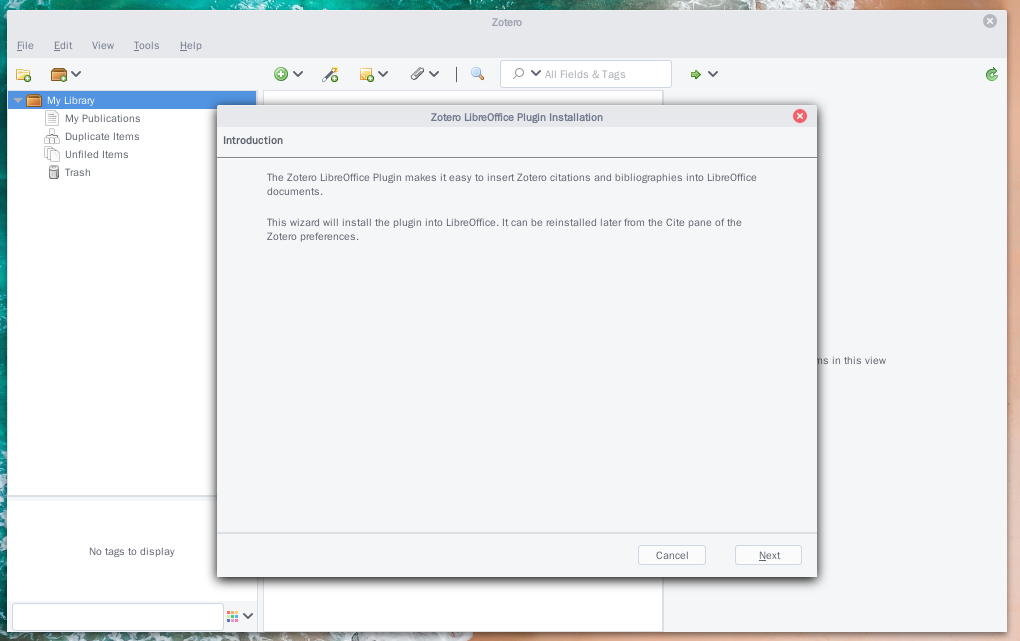
\includegraphics[width=.9\textwidth]{imgs/sp2_zotero_app_started.png}
    \caption{Вікно програми Zotero при запуску застосунку.}
    \label{pic:zotero-app-started}
\end{figure}

\begin{figure}[H]
    \centering
    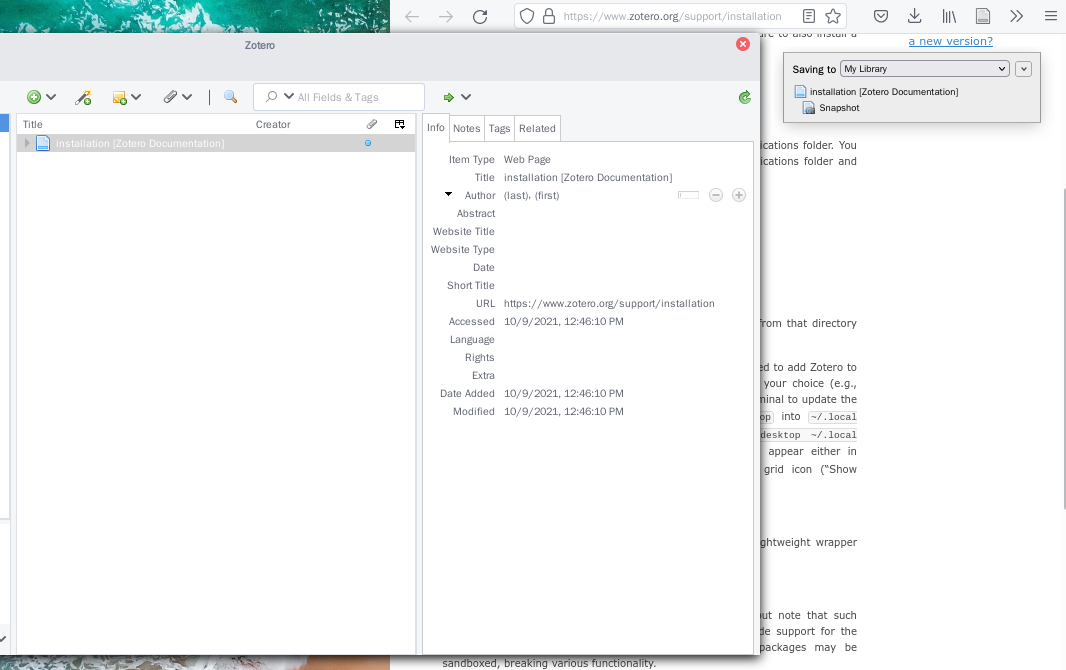
\includegraphics[width=.9\textwidth]{imgs/sp2_zotero_connector.png}
    \caption{Браузерне розширення Zotero пов'язується із десктопною аплікацією.}
    \label{pic:zotero-connector}
\end{figure}

За умовами завдання я додав необхідну кількість публікацій до бібліографії. Сформований список показано на Рис.~\ref{pic:citation-list}.

\begin{figure}[h]
    \centering
    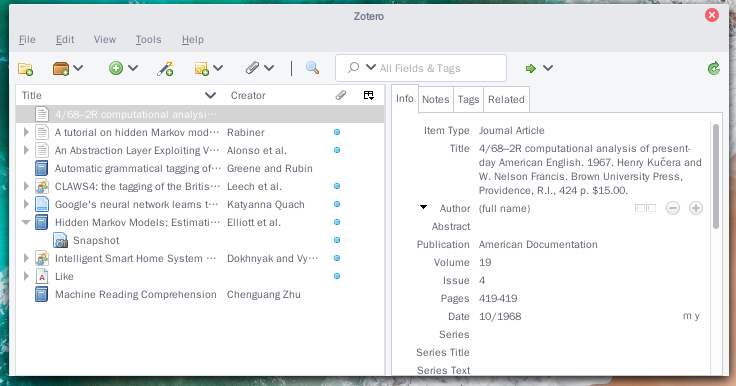
\includegraphics[width=.9\textwidth]{imgs/sp2_citation_list.png}
    \caption{Сформована бібліографія.}
    \label{pic:citation-list}
\end{figure}

Якщо стаття переноситься неправильно, відомості про неї можна відредагувати вручну. Процес перегляду та редагування відомостей показано на Рис.~\ref{pic:kucera-fields}.

\begin{figure}[t]
    \centering
    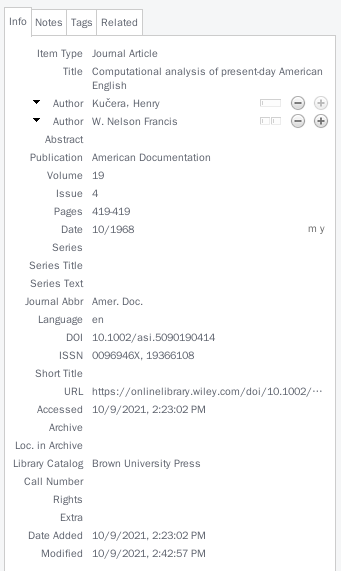
\includegraphics[width=8cm]{imgs/sp2_kucera_fields.png}
    \caption{Перегляд відомостей для статті Генрі Кучери.}
    \label{pic:kucera-fields}
\end{figure}

\Subsection{Текст за темою роботи}

Далі подано приклад тексту з посиланнями в стилі APA 7\textsuperscript{th}. Звичайно, вигляд посилань всередині тексту відрізнятиметься при використанні різних стилей. Окрім тієї кількості посилань, яка вимагається у завданні практичної, я додав також свої.

Проблему розмітки частини мови у тексті можна вважати однією з базових в обробці природних мов. Можливість розпізнавання частини мови відкриває нам шлях до синтаксичного аналізу, аналізу тональності і навіть машинного перекладу (Chenguang, 2021). Якщо задачу машинного перекладу зараз набагато ефективніше вирішують з допомогою нейронних мереж (Quach, 2016), то синтаксичний аналіз потрібен у всіх випадках, коли машина повинна \flqq{}зрозуміти\frqq{} текст, і навіть якось відповідати на нього. Найпоширенішим прикладом такого аналізатора є голосові помічники (Alonsom, 2021) (Dokhnyak, 2021), що зараз вбудовані у багато операційних систем та розробляються корпораціями на кшталт Google, Microsoft та Apple. У мовах, де слово, переходить між частинами мови набагато вільніше, ніж в українській, розмітка слів також відіграє роль усунення неоднозначностей. Наприклад, речення англійською \flqq{}I like you\frqq{} при аналізі тональності може бути класифікованим як таке, що має позитивнішу емоцію, ніж \flqq{}you're like me\frqq{} -- хоч вони дуже схожі символьно, слово \flqq{}like\frqq{} несе зовсім іншу емоцію, позаяк належить до різних частин мови в цих контекстах.

Перші систематичні роботи у цьому напрямку розпочались у 60-их роках минулого століття зі створенням Браунівського корпусу англійської мови Нельсоном Франсисом та Генрі Кучера (Kučera, 1968). Він поділений на 15 розділів (репортажі, огляди, релігія, наука тощо) та містить приблизно мільйон слів. На основі цього корпусу створювали програми, які задля розмітки частини мови використовували вручну створені правила (наприклад, \textit{\flqq{}найбільш ймовірно, що слово після прикметника -- іменник або дієслово\frqq{}}, \textit{\flqq{}після прийменника ніколи не йде дієслово\frqq{}}). Такі програми давали лише 70\% точності (Greene, 1971), і це був найкращий результат аж до спроби використати для такої задачі приховану модель Маркова у 80-их роках. В цей же час виходить стаття Рабінера Ловренса з описом алгоритмів, що можуть бути застосовані на ПММ (Rabiner, 1989). Створена з використанням цієї моделі програма CLAWS досягала точності до 93-95\% (Leech, 1994).

Окрім спроб вирішення цієї задачі за допомогою навчання без вчителя, з того часу нічого не змінилось. Прихована марковська модель і досі вважається найбільш простим та надійним підходом при визначенні частини мови (Elliott, 1995). І дійсно, вона дуже вдало описує процес створення осмислених наборів інформації. Мовець (або той, хто пише) думає абстракціями, у нього означення межує з означуваним, прийменник із ціллю, а числівник із предметами; у мовця одна думка перетікає в іншу, а потім він обрамлює це у слова. Слова мовця можна вважати спостереженнями марковської моделі, а частини мови -- прихованими станами, що перетікають з одного в інший. Спеціально для відновлення послідовності невідомих прихованих станів на основі спостережень існує алгоритм Вітербі.

\Subsection{Цитування у стилі APA 7\textsuperscript{th}}

\begin{hangparas}{3em}{1}

Alonso, R., Concas, E., \& Reforgiato Recupero, D. (2021). An Abstraction Layer Exploiting Voice Assistant Technologies for Effective Human—Robot Interaction. \textit{Applied Sciences}, 11(19), 9165. \url{https://doi.org/10.3390/app11199165}

Chenguang Zhu. (2021). \textit{Machine Reading Comprehension} (1-ше вид.). Elsevier. \url{https://doi.org/10.1016/C2020-0-03297-4}

Dokhnyak, B., \& Vysotska, V. (2021). Intelligent Smart Home System Using Amazon Alexa Tools. В M. Emmerich, V. Lytvyn, V. Vysotska, V. Basto-Fernandes, \& V. Lytvynenko (Ред.), \textit{Modern Machine Learning Technologies and Data Science Workshop. Proc. 3rd International Workshop (MoMLeT\&DS 2021).  Volume I: Main Conference} (Вип. 2917, с. 441–464). CEUR. \url{http://ceur-ws.org/Vol-2917/#paper33}

Elliott, R. J., Aggoun, L., \& Moore, J. B. (1995). \textit{Hidden Markov Models: Estimation and Control.} Springer-Verlag. \url{https://doi.org/10.1007/978-0-387-84854-9}

Greene, B. B., \& Rubin, G. M. (1971). \textit{Automatic grammatical tagging of English}. Dept. of Linguistics, Brown University.

Katyanna Quach. (2016, Листопад 17). \textit{Google’s neural network learns to translate languages it hasn’t been trained on • The Register.} The Register. \url{https://www.theregister.com/2016/11/17/googles\_neural\_net\_translates\_languages\_not\_trained\_on/}

Kučera, H. \& W. Nelson Francis. (1968). Computational analysis of present-day American English. \textit{American Documentation}, 19(4), 419–419. \url{https://doi.org/10.1002/asi.5090190414}

Leech, G., Garside, R., \& Bryant, M. (1994). CLAWS4: The tagging of the British National Corpus. \textit{Proceedings of the 15th Conference on Computational Linguistics}, 1, 622. \url{https://doi.org/10.3115/991886.991996}

Rabiner, L. R. (1989). A tutorial on hidden Markov models and selected applications in speech recognition. \textit{Proceedings of the IEEE}, 77(2), 257–286. \url{https://doi.org/10.1109/5.18626}

\end{hangparas}

\Subsection{Цитування у стилі Vancouver}

При цитуванні у стилі Vancouver посилання всередині тексту можна проставляти всередині квадратних дужок (наприклад: \flqq{}\textit{[1]}\frqq{}). Також всередині дужок можна проставити потрібну сторінку (наприклад: \flqq{}\textit{[1 с23]}\frqq{}) \cite{monash}.

Далі подано вигляд бібліографії.

1.  Rabiner LR. A tutorial on hidden Markov models and selected applications in speech recognition. Proceedings of the IEEE. Лютий 1989;77(2):257–86.

2.  Alonso R, Concas E, Reforgiato Recupero D. An Abstraction Layer Exploiting Voice Assistant Technologies for Effective Human—Robot Interaction. Applied Sciences. Січень 2021;11(19):9165. 

3.  Greene BB, Rubin GM. Automatic grammatical tagging of English. Providence, R.I.: Dept. of Linguistics, Brown University; 1971. 

4.  Leech G, Garside R, Bryant M. CLAWS4: the tagging of the British National Corpus. В: Proceedings of the 15th conference on Computational linguistics - [Інтернет]. Kyoto, Japan: Association for Computational Linguistics; 1994 [цит. за 09, Жовтень 2021]. с. 622. Доступний у: \url{http://portal.acm.org/citation.cfm?doid=991886.991996}

5.  Kučera H, W. Nelson Francis. Computational analysis of present-day American English. Amer Doc. Жовтень 1968;19(4):419–419. 

6.  Katyanna Quach. Google’s neural network learns to translate languages it hasn’t been trained on • The Register [Інтернет]. The Register. 2016 [цит. за 09, Жовтень 2021]. Доступний у: \url{https://www.theregister.com/2016/11/17/googles\_neural\_net\_translates\_languages\_not\_trained\_on/}

7.  Elliott RJ, Aggoun L, Moore JB. Hidden Markov Models: Estimation and Control [Інтернет]. New York: Springer-Verlag; 1995 [цит. за 09, Жовтень 2021]. (Stochastic Modelling and Applied Probability). Доступний у: \url{https://www.springer.com/gp/book/9780387943640}

8.  Dokhnyak B, Vysotska V. Intelligent Smart Home System Using Amazon Alexa Tools. В: Emmerich M, Lytvyn V, Vysotska V, Basto-Fernandes V, Lytvynenko V, за ред. Modern Machine Learning Technologies and Data Science Workshop Proc 3rd International Workshop (MoMLeT\&DS 2021) Volume I: Main Conference [Інтернет]. Lviv-Shatsk, Ukraine: CEUR; 2021 [цит. за 09, Жовтень 2021]. с. 441–64. (CEUR Workshop Proceedings; вип. 2917). Доступний у: \url{http://ceur-ws.org/Vol-2917/#paper33}

9.     Chenguang Zhu. Machine Reading Comprehension [Інтернет]. 1st вид. Elsevier; 2021 [цит. за 09, Жовтень 2021]. 270 с. Доступний у: \url{https://linkinghub.elsevier.com/retrieve/pii/C20200032974}

\Subsection{Цитування у стилі ACM Computing Surveys}

Для додавання цього стилю до застосунку Zotero я використав пошук по репозиторію стилів. Процес додавання продемонстровано на Рис.~\ref{pic:adding-acm-comp-surv}

\begin{figure}[H]
    \centering
    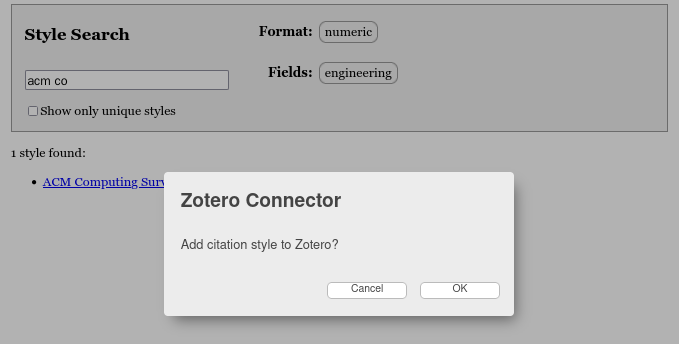
\includegraphics[width=.8\textwidth]{imgs/sp2_adding_acm_comp_surv.png}
    \caption{Додавання стилю ACM Computing Survey.}
    \label{pic:adding-acm-comp-surv}
\end{figure}

Стиль посилань у тексті при використанні цього стилю такий самий, як і при використанні стилю Vancouver. Далі подана оформлена бібліографія.

\begin{hangparas}{1.7em}{1}

[1] Ruben Alonso, Emanuele Concas, and Diego Reforgiato Recupero. 2021. An Abstraction Layer Exploiting Voice Assistant Technologies for Effective Human—Robot Interaction. \textit{Applied Sciences} 11, 19 (January 2021), 9165. DOI:\url{https://doi.org/10.3390/app11199165}

[2] Chenguang Zhu. 2021. \textit{Machine Reading Comprehension} (1st ed.). Elsevier. DOI:\url{https://doi.org/10.1016/C2020-0-03297-4}

[3] Bohdan Dokhnyak and Victoria Vysotska. 2021. Intelligent Smart Home System Using Amazon Alexa Tools. \textit{In Modern Machine Learning Technologies and Data Science Workshop. Proc. 3rd International Workshop (MoMLeT\&DS 2021)}. Volume I: Main Conference (CEUR Workshop Proceedings), CEUR, Lviv-Shatsk, Ukraine, 441–464. Retrieved October 9, 2021 from \url{http://ceur-ws.org/Vol-2917/#paper33}

[4] Robert J. Elliott, Lakhdar Aggoun, and John B. Moore. 1995. \textit{Hidden Markov Models: Estimation and Control.} Springer-Verlag, New York. DOI:\url{https://doi.org/10.1007/978-0-387-84854-9}

[5] Barbara B Greene and Gerald M Rubin. 1971. \textit{Automatic grammatical tagging of English}. Dept. of Linguistics, Brown University, Providence, R.I.

[6] Katyanna Quach. 2016. Google’s neural network learns to translate languages it hasn’t been trained on • The Register. \textit{The Register}. Retrieved October 9, 2021 from \url{https://www.theregister.com/2016/11/17/googles\_neural\_net\_translates\_languages\_not\_trained\_on/}

[7] Henry Kučera and W. Nelson Francis. 1968. Computational analysis of present-day American English. \textit{Amer. Doc.} 19, 4 (October 1968), 419–419. DOI:\url{https://doi.org/10.1002/asi.5090190414}

[8] Geoffrey Leech, Roger Garside, and Michael Bryant. 1994. CLAWS4: the tagging of the British National Corpus. In \textit{Proceedings of the 15th conference on Computational linguistics} -, Association for Computational Linguistics, Kyoto, Japan, 622. DOI:\url{https://doi.org/10.3115/991886.991996}

[9] L.R. Rabiner. 1989. A tutorial on hidden Markov models and selected applications in speech recognition. \textit{Proceedings of the IEEE 77}, 2 (February 1989), 257–286. DOI:\url{https://doi.org/10.1109/5.18626}

\end{hangparas}

\Section{Результати та висновки}

У межах цієї практичної роботи я встановив, налаштувався та навчився використовувати безкоштовний бібліографічний менеджер Zotero для оформленя списку літератури у наукових роботах. В процесі виконання виявилось, що цей менеджер має деякі недоліки. Далі подано перелік.

\begin{itemize}
    \item При перегляді потрібної праці на сторінці Elsevier розширені опції імпорту відсутні. Доступний лише імпорт web-сторінки. Зрозуміло, що таке посилання ніякої наукової цінності не несе. Цю проблему можна вирішити, якщо натиснути на посилання \flqq{}переглянути на ScienceDirect\frqq{}, і спробувати імпортувати звідти.
    \item При імпорті публікації з деяких джерел Zotero розпізнає не всі дані. Наприклад, не додається кількість сторінок, опис та автор роботи. Ці дані доводиться додавати вручну. У мене ця проблема трапилась, коли я намагався додати публікацію лише за відомим посиланням на doi.org.
    \item Zotero не розпізнає автора статті та іншу важливу інформацію при імпорті звичайних Web-сторінок.
    \item При імпорті книжок з ScienceDirect менеджер розпізнає розділи книги як окремі праці, і можна помилково імпортувати їх усі. Цей випадок продемонстровано на Рис.~\ref{pic:too-many-sections-elsevier}.
    \item Менеджер використовує синхронізацію із сервером. Це чудова опція, однак у мене траплялись випадки, коли я видаляв деякі записи з колекції, але потім вони підвантажувались назад.
\end{itemize}

\begin{figure}[H]
    \centering
    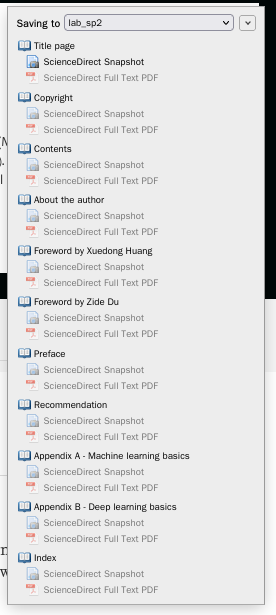
\includegraphics[width=7cm]{imgs/sp2_too_many_sections_elsevier.png}
    \caption{Помилково додані розділи книги як окремі праці.}
    \label{pic:too-many-sections-elsevier}
\end{figure}

При написанні власної праці я використовую інші інструменти. Наприклад, в мережі доступна безкоштовна утиліта Grafiati, яка не вимагає жодного встановлення абощо, і у безкоштовній версії дозволяє додавати до 100 записів, форматувати їх згідно вимог ВАК (і багатьох інших стилів) та сортувати по алфавіту. Пізніше ці записи можна додати до оточення \texttt{thebibliography} у Latex, і посилатись на потрібні записи за допомогою команди \texttt{\textbackslash{}cite}. При використанні пакету \texttt{hyperref} можна створити інтерактивний PDF документ, де натискання на певне посилання у тексті відправлятиме користувача на відповідний запис у бібліографії.

\Section{Список використаної літератури}

\begingroup
\renewcommand{\section}[2]{}
\renewcommand{\chapter}[2]{}
\begin{thebibliography}{99}
\bibitem{publ} Цитати у науковій статті: поради як правильно їх оформлювати [Електронний ресурс] – Режим доступу: \url{https://ua.publ.science/uk/blog/tsitaty-v-nauchnoy-statye-sovety-kak-pravilno-ikh-oformlyat} (відвідано 17.10.2020)
\bibitem{ieee} IEEE Xplore Digital Library [Електронний ресурс] – Режим доступу: \url{https://ieeexplore.ieee.org/Xplore/home.jsp} (відвідано 17.10.2020) 
\bibitem{monash} Quick reference guide for Vancouver Citing \& Referencing style [Електронний ресурс] // Subject guides at Monash University. – Режим доступу: \url{https://guides.lib.monash.edu/ld.php?content\_id=48260115} (дата звернення: 09.10.2021). – Назва з екрана.
\bibitem{zotero} Zotero Style Repository [Електронний ресурс] – Режим доступу: \url{https://www.zotero.org/styles} (відвідано 17.10.2020)
\end{thebibliography}

\end{document}
